% Last Update: 2025.01.23 by Tetsuaki Baba
% Last Update: 2024.01.28 by Tetsuaki Baba

% 学部は \documentclass[a4paper,uplatex]{jsarticle}を利用して,\section で論文を構成してください.
% 修士、博士は \documentclass[a4paper,uplatex]{jsreport} を利用して, \chapter で論文を構成してください.
% for English users: replace jsarticle -> article or jsreport -> report
\documentclass[a4paper,uplatex]{jsarticle}
\usepackage{fix-cm}

% 必要なパッケージを読み込み(ここはいじらない)%%%%%
\usepackage{iathesis}
\usepackage[dvipdfmx]{graphicx,xcolor}
\usepackage{listings}
\usepackage{fancyvrb}
\usepackage{appendix}
\usepackage[utf8]{inputenc}
\usepackage{csquotes}
\usepackage[english]{babel}
%%%%%%%%%%%%%%%%%%%%%%%%%%%%%%%%%%%%%%%%%

% 文献引用設定 %%%%%%%%%%%%%%%%%%%%%%%%%%%
% Default: [文献番号] スタイル sorting=none: 文献が論文中に登場する順序.このほか,nty, nyt等ある.sort オプションについては 次のリンクを参照する https://ja.overleaf.com/learn/latex/Bibliography_management_with_biblatex#Reference_guide
\usepackage[backend=biber,style=numeric,sorting=none]{biblatex}

% 著者名(西暦)スタイル style=authoryearの場合は引用表記が「名,姓」の順になるので,bib内のauthorを修正すること
% \usepackage[backend=biber,style=numeric,sorting=none]{biblatex}

% 文献読み込み
\addbibresource{references.bib}
%%%%%%%%%%%%%%%%%%%%%%%%%%%%%%%%%%%%%%%%

\usepackage{url}
\urlstyle{same}

\usepackage{tikz}
\usetikzlibrary{positioning, shapes, arrows.meta, calc, fit}

\lstdefinelanguage{json}{
    basicstyle=\normalfont\ttfamily,
    numbers=left,
    numberstyle=\scriptsize,
    stepnumber=1,
    numbersep=8pt,
    showstringspaces=false,
    breaklines=true,
    frame=lines,
    backgroundcolor=\color{white},
    literate=
     *{0}{{{\color{blue}0}}}{1}
      {1}{{{\color{blue}1}}}{1}
      {2}{{{\color{blue}2}}}{1}
      {3}{{{\color{blue}3}}}{1}
      {4}{{{\color{blue}4}}}{1}
      {5}{{{\color{blue}5}}}{1}
      {6}{{{\color{blue}6}}}{1}
      {7}{{{\color{blue}7}}}{1}
      {8}{{{\color{blue}8}}}{1}
      {9}{{{\color{blue}9}}}{1}
      {:}{{{\color{red}{:}}}}{1}
      {,}{{{\color{red}{,}}}}{1}
      {\{}{{{\color{blue}{\{}}}}{1}
      {\}}{{{\color{blue}{\}}}}}{1}
      {[}{{{\color{blue}{[}}}}{1}
      {]}{{{\color{blue}{]}}}}{1},
}

\usepackage{CJKutf8}

\begin{document}

% ソースコード表記は code_listings.tex を参照してください。詳細:https://www.overleaf.com/learn/latex/Code_listing

%New colors defined below
\definecolor{codegreen}{rgb}{0,0.6,0}
\definecolor{codegray}{rgb}{0.5,0.5,0.5}
\definecolor{codepurple}{rgb}{0.58,0,0.82}
\definecolor{backcolour}{rgb}{0.95,0.95,0.92}

% JavaScript
\lstdefinelanguage{JavaScript}{
  morekeywords={typeof, new, true, false, catch, function, return, null, catch, switch, var, if, in, while, do, else, case, break},
  morecomment=[s]{/*}{*/},
  morecomment=[l]//,
  morestring=[b]",
  morestring=[b]'
}

% CSS
\lstdefinelanguage{CSS}{
  keywords={color,background-image:,margin,padding,font,weight,display,position,top,left,right,bottom,list,style,border,size,white,space,min,width, transition:, transform:, transition-property, transition-duration, transition-timing-function},	
  sensitive=true,
  morecomment=[l]{//},
  morecomment=[s]{/*}{*/},
  morestring=[b]',
  morestring=[b]",
  alsoletter={:},
  alsodigit={-}
}

\lstdefinelanguage{HTML5}{
  language=html,
  sensitive=true,	
  alsoletter={<>=-},	
  morecomment=[s]{<!-}{-->},
  tag=[s],
  otherkeywords={
  % General
  >,
  % Standard tags
	<!DOCTYPE,
  </html, <html, <head, <title, </title, <style, </style, <link, </head, <meta, />,
	% body
	</body, <body,
	% Divs
	</div, <div, </div>, 
	% Paragraphs
	</p, <p, </p>,
	% scripts
	</script, <script,
  % More tags...
  <canvas, /canvas>, <svg, <rect, <animateTransform, </rect>, </svg>, <video, <source, <iframe, </iframe>, </video>, <image, </image>, <header, </header, <article, </article
  },
  ndkeywords={
  % General
  =,
  % HTML attributes
  charset=, src=, id=, width=, height=, style=, type=, rel=, href=,
  % SVG attributes
  fill=, attributeName=, begin=, dur=, from=, to=, poster=, controls=, x=, y=, repeatCount=, xlink:href=,
  % properties
  margin:, padding:, background-image:, border:, top:, left:, position:, width:, height:, margin-top:, margin-bottom:, font-size:, line-height:,
	% CSS3 properties
  transform:, -moz-transform:, -webkit-transform:,
  animation:, -webkit-animation:,
  transition:,  transition-duration:, transition-property:, transition-timing-function:,
  }
}

%Code listing style named "mystyle"
\lstdefinestyle{mystyle}{
  backgroundcolor=\color{backcolour}, commentstyle=\color{codegreen},
  keywordstyle=\color{magenta},
  numberstyle=\tiny\color{codegray},
  stringstyle=\color{codepurple},
  basicstyle=\ttfamily\footnotesize,
  breakatwhitespace=false,         
  breaklines=true,                 
  captionpos=b,                    
  keepspaces=true,                 
  numbers=left,                    
  numbersep=5pt,                  
  showspaces=false,                
  showstringspaces=false,
  showtabs=false,                  
  tabsize=2
}
\lstset{style=mystyle}

% settings for kind of thesis %%%%%%%
% 卒業論文の場合は \bachelorthesis
% 卒業作品の場合は \bacheloarthesisartwork
% 修士論文の場合は \masterthesis
% 博士論文の場合は \doctorthesis
% For English Users
% 卒業論文の場合は \bachelorthesisEN
% 卒業作品の場合は \bacheloarthesisartworkEN
% 修士論文の場合は \masterthesisEN
% 博士論文の場合は \doctorthesisEN
\bachelorthesis % このサンプルでは卒業論文にしています
%%%%%%%%%%%%%%%%%%%%%%%%%%%%%%%%%%%%%

% 表紙 %%%%%%%%%%%%%%%%%%%%%%%%%%%%%%%
% for English users, Please replace Japanese words into English
% \title{一点物売買プラットフォームの機能に対する動作検証を目的とした社会的シナリオに則ったデータ生成エージェントの開発}
\title{一点物売買プラットフォームの動作検証を目的とした社会的シナリオに則ったデータ生成エージェントの開発}
\fisicalyear{ \currentfisicalyear 年度}
%\fisicalyear{ FY \currentfisicalyear }
\supervisor{指導教員}{植松 幸生 准教授} % 氏名欄に指導教員名を入れる
\studentNumber{6322087}
\author{三笠 悠太郎} % 自分の氏名
\affiliation{東京理科大学 創域理工学部 情報計算科学科} % 大学院は以下のコメントアウトした所属を参照
% \affiliation{東京都立大学大学院\\システムデザイン研究科 博士前期課程\\インダストリアルアート学域}
% \affiliation{Master's Course\\Division of Industrial Art\\Graduate School of Systems Design\\Tokyo Metropolitan University}

\submissiondate{ \currentyear 年2月15日} % 実際の論文提出日にすること
\maketitle
%%%%%%%%%%%%%%%%%%%%%%%%%%%%%%%%%%%%%

\pagenumbering{roman} % 要旨はRoman書体で表示
\setcounter{page}{1} % 1から振り直す

% 副題がある場合は必ず先頭にハイフン(半角)を3つつけること
\jasummary{一点物売買プラットフォームの動作検証を目的とした社会的シナリオに則ったデータ生成エージェントの開発}{}

% 本研究では,一点物売買プラットフォームの開発を行っている.本プラットフォームは,作品の背景にあるストーリーや,クリエイターとコミュニティの社会的関係性を表現することを特徴としており,これをシステム上で実現するために,データベースのリレーション構造は社会的シナリオを反映して複雑化している.このようなサービスの開発初期段階において,システムのUI表示や検索システムの有用性のような,多数のデータが存在する状況が必要な機能を適切に検証するためには,サービス固有の複雑なデータ構造上で整合性を保ったテストデータが不可欠である.しかし,社会的シナリオを反映したデータを手動で大量に用意することは困難であり,従来のランダムなダミーデータ生成手法では,リレーションの整合性やコンテンツの意味的な文脈を再現できないという課題があった.

近年,クリエイターエコノミーの発展に伴い,作品単体の価値だけでなく,その背景にあるストーリーやクリエイターとファンが形成するコミュニティの文脈を統合して流通させるWebプラットフォームの重要性が高まっている.このようなプラットフォームにおいて,ユーザー間の社会的相互作用や共同制作プロジェクトといった関係性を記録・表現する必要があるため,そのデータベースは社会的シナリオを反映した複雑なリレーション構造となる傾向にある.このようなプラットフォームの開発初期段階において,UI表示や検索システムの有用性を検証するためには,サービス固有のデータ構造と整合性を保った大量のテストデータが不可欠である.しかしながら,社会的シナリオを反映したデータを手動で大量に用意することは困難であり,従来のランダムなダミーデータ生成手法では,リレーションの整合性やコンテンツの意味的な文脈を再現できないという課題があった.

% :LATEST
本研究では,大規模言語モデル(LLM)を用いて,ユーザの社会的背景や文脈を記述した社会的シナリオを構築し,それに基づいてサービス固有のリレーションを持つデータ群を生成するエージェントを開発した.本エージェントは,LangGraphを用いたステートマシンとして設計されており,データベースを活用した記憶機構を実装している.これにより,過去に生成したデータと重複しない多様なコンセプトを立案し,そのコンセプトに基づいて相互に整合性の取れたユーザー,プロジェクト,作品群をひとまとまりの単位として,本プラットフォーム上のデータ構造に特化した,自律的にデータを生成・投入する能力を持つデータ生成エージェントを開発した.

提案手法の有効性を検証するため,実験環境として一点物取引に特化したWebプラットフォームを開発し,google, Open AIの4つの基盤モデルに対して本エージェントを適用して1000件のデータ生成実験を行った.評価の結果,過去の生成履歴を参照する記憶機構を導入することで,Gemini 3 Flashにて生成される語彙数が39.0\%増加し,GPT-5.2においては全生成データのコサイン類似度分布が効果量 $d=-0.51$ で低下した.これらの結果は,記憶機構が生成内容の重複や特定のパターンへの収束を抑制し,生成されるデータセット全体の多様性を向上させることを示している.本研究は,LLMを用いた社会的シナリオ生成が,開発初期段階においても実運用環境に近い整合性と多様性を持つテストデータの生成に有効であることを実証した.

\summary{Title}{--- Subtitle}
The author shall describe his/her thesis in English text. 150 words.

% 目次表示の深さ設定 %%%%%%%%%%%%%%%%%%%%%%%%%
% 以下をコメントアウトすると,subsubsectionまで目次に表示される.数字を減らすと浅く,増やすと深くなる
% \setcounter{tocdepth}{3}
%%%%%%%%%%%%%%%%%%%%%%%%%%%%%%%%%%%%%%%%%%%
\makemokuji % 目次の作成

\newpage % 改ページ

% フッターのページ設定 %%%%%%%%%%%%%%%%%%%%%%%%%
\pagenumbering{arabic}  % 論文本体はArabicで表示
\setcounter{page}{1} % ページ番号を1から振り直す
\pagestyle{plain}
%%%%%%%%%%%%%%%%%%%%%%%%%%%%%%%%%%%%%%%%%%%

% 章の読み込み
\section{序論}
\label{chap:introduction}

\subsection{背景}

\subsubsection{クリエイターエコノミーの拡大と作品流通の変容}
近年,インターネット技術の発展とソーシャルネットワーキングサービスの普及により,個人が自身の創作物を発信・販売し,収益を得るクリエイターエコノミーが急速に拡大している\cite{goldman2023creator}.動画投稿,ライブ配信,ハンドメイド作品の販売,デジタルコンテンツの提供など,その形態は多岐にわたり,従来は企業や専門家が独占していた生産・流通・販売のプロセスが個人レベルまで民主化された.

特に,物理的な創作物を制作するクリエイターにとって,Mercari \cite{mercari} やminne \cite{minne} といったCtoCマーケットプレイスの普及,あるいはBASE \cite{base} のように個人が手軽に独自のオンラインストアを開設できるサービスの登場は,販路開拓のハードルを劇的に引き下げた.
中でも,イラストや同人誌などのサブカルチャー領域に特化したBOOTH \cite{booth} は,物理的な作品とデジタルコンテンツを並列して扱うことができ,本研究が対象とするような「作品の文脈」を重視するクリエイター層から厚い支持を得ている.
これにより,趣味の延長線上で制作を行っていた個人が,容易に売り手として市場に参加できる環境が整った.

しかし,これらの既存プラットフォームの多くは,既製品や大量生産品,あるいは不用品の流通に最適化されて設計されている側面が強い.商品自体は代替可能な商品として扱われ,その背後にある制作者の思想,制作過程の試行錯誤,作品が生まれた文脈は,商品説明欄の補助的なテキスト情報として扱われるに留まる.

一点物や極めて少数の生産数しか持たない創作物において,その価値の源泉は物理的な素材や機能性よりも,この物語にこそ存在する.既存のプラットフォームでは,こうした作品固有の物語性や文脈を十分に表現・保存することが難しく,結果として作品が単なる商品として消費され,制作者のブランディングや持続的なファンコミュニティの形成に繋がりにくいという課題がある.

\subsubsection{物理的な展示・即売会における制約とアーカイブの欠如}
デジタルプラットフォームの対極として,学園祭,展示会,即売会といった物理的な場での作品発表も依然として重要な役割を果たしている.これらの場は,制作者と鑑賞者が直接交流し,作品の熱量を共有できる貴重な機会である.

しかし,物理的なイベントには一過性という避けられない制約が存在する.
第一に,展示情報のアーカイブ化の問題である.展示会のために制作された解説パネルやキャプションボードは,イベント終了とともに廃棄または散逸することが多く,そこに記された詳細な作品情報はデジタル空間に蓄積されない.結果として,イベントに参加できなかった潜在的なファンには作品の魅力が届かず,制作者のポートフォリオとしても十分に機能しない場合が多い.

第二に,金銭授受と販売機会の損失である.学園祭や小規模な展示会では,販売機能を持たず展示のみとするケースや,販売する場合でも現金取引のみの対応となるケースが多い.また,展示されている作品そのものを購入したいという需要があっても,会期終了後の引き渡し手続きや配送手配の煩雑さから,その場での成約に至らないことも頻繁に発生する.このように,物理的な展示空間とデジタル上の決済・物流システムが分断されていることにより,多くの経済的機会が損失しているのが現状である.

\subsubsection{一点物取引における価格決定と信頼性の課題}
一点物,あるいは極めて供給量の少ない作品の流通においては,価格決定メカニズムと取引の信頼性に関して特有の課題が存在する.

まず,価格決定においては,需要が供給を大幅に上回る場合,定価販売形式では早い者勝ちとなり,転売目的の購入や,botによる自動購入などの問題を引き起こしやすい.これに対し,オークション形式は需要に応じた適正価格を発見する有効な手段であるが,既存のオークションサイトは,前述の通り不用品処分の文脈が強く,クリエイターが自身の作品を発表・販売する場としてのブランディング機能に欠ける場合がある.

\subsubsection{共同体による創作活動と収益分配の複雑性}
創作活動は必ずしも個人だけで完結するものではない.サークル活動,合同誌,アンソロジー企画,YouTuber同士のコラボレーションなど,複数のクリエイターが関与するプロジェクト単位での活動も一般的である.
しかし,既存のCtoCプラットフォームの多くは一人の売り手対一人の買い手という単純な取引モデルを前提としている.そのため,一つの作品またはイベントから得られた収益を,関与した複数のメンバーに分配する場合,代表者が一度全額を受け取り,その後銀行振込などで個別に再分配するという,極めてアナログで煩雑な事務作業が必要となる.これは,企画主催者の負担を増大させ,継続的な共同制作活動を阻害する要因となっている.



\subsection{開発上の課題:複雑な文脈を持つシステムの検証難易度}
前述したような作品の物語や複雑な権利・収益構造を持つプラットフォームを新規に開発する際,最大の障壁となるのが検証用データの不足である.

一般的なECサイト(商品と価格のみの管理)であれば,ランダムな文字列やダミー画像を用いた機械的なデータ生成(Faker.js \cite{fakerjs} 等)で十分に機能検証が可能である.
しかし,本研究が対象とするような文脈を重視するシステムにおいては,以下の理由により,既存のテストデータ生成手法が通用しない.

\begin{enumerate}
	\item \textbf{リレーションの整合性}: プロジェクト主催者と参加メンバー,そして出品された作品の間には,矛盾のない論理的な関係性が求められる.ランダム生成では,「部外者が他人のプロジェクトの作品を管理している」といった矛盾が頻発し,権限管理ロジックのテストが成立しない.
	\item \textbf{検索・推薦アルゴリズムの検証}: 文脈に基づく検索システムを評価するには,データ自体に意味のあるテキスト(制作背景や動機)が含まれている必要がある.Lorem Ipsumのような無意味なテキストでは,検索精度の検証が不可能である.
	% \item \textbf{コールドスタート問題}: 近年のAIを用いたデータ生成手法は,既存の大量のデータを学習元として必要とする.しかし,新規サービスの開発初期段階(0 $\to$ 1フェーズ)においては,学習すべき正解データそのものが存在しない.
\end{enumerate}

したがって,開発者は「手動で時間をかけて整合性のあるデータを作る」か,「質の低いデータで妥協して検証を行う」かの二者択一を迫られており,これが開発効率と品質向上のボトルネックとなっていた.

\subsection{本研究の目的}
本研究の目的は,一点物売買プラットフォームの開発と,それを支える新たなテストデータ生成手法の確立の2点にある.

\subsubsection{一点物作品のナラティブを保存するプラットフォームの開発}
第一に,既存のEコマースでは埋没しがちな作品の文脈を構造化データとして保存・活用できる,新たなCtoCプラットフォームを構築する(第4章にて詳述).これは本研究において,提案するデータ生成手法の有効性を検証するための実験環境としての役割も担う.

\subsubsection{LLMを用いた社会的シナリオ生成によるシステム検証}
第二の,そして本論文の主眼となる目的は,上記のような複雑なリレーションを持つWebサービスの開発において,大規模言語モデル(LLM)を活用した社会的シナリオに基づくテストデータ生成手法を提案・実証することである.

本研究では,LLMに「架空のユーザーの人格」や「プロジェクトの動機」といった社会的背景(社会的シナリオ)を与え,自律的にデータベースへの登録を行わせるエージェントシステムを構築する.
さらに,エージェントに記憶機構(RAG)を組み込むことで,既存データとの衝突を回避し,多様なシナリオを生成できるかを実験的に検証する.
これにより,学習データが存在しない環境下においても,あたかも人間が実際に活動しているかのような,高密度で整合性の取れたテストデータを大量生成できることを示す.

\section{関連研究}
\label{chap:related_work}

本章では,ソフトウェアテストデータの生成手法,大規模言語モデル(LLM)のデータ生成への応用に関する先行研究を概観し,本研究の位置づけを明確にする.

\subsection{ソフトウェアテストデータの生成手法}
% 2.1 ルールベースおよびランダムサンプリングによるデータ生成
Webアプリケーションの開発現場において,動作検証や負荷試験のためのテストデータ生成は不可欠な工程であり,主に構文的整合性やコード網羅率の確保に主眼が置かれてきた\cite{edvardsson1999survey}.

代表的なアプローチとして,Faker.js \cite{fakerjs} や JavaFaker \cite{javafaker} に代表されるライブラリを用いたランダム生成手法が存在する.これらは,正規表現や定義済みの辞書に基づき,氏名,住所,メールアドレスといった形式が決まったデータを大量に生成することに長けている.
また,Mockaroo \cite{mockaroo} のようなデータ生成サービスでは,GUI上でスキーマ定義を行うことで,ある程度の外部キー制約を満たしたCSVやSQLデータを生成可能である.
さらに,近年のWeb開発フレームワーク(例:Prisma \cite{prisma} などのORM)には,開発初期のシードデータ(初期データ)を投入する機能が標準で備わっていることが多いが,これらも基本的には開発者が手動で作成した固定データか,あるいは前述のFaker等で生成したランダムデータを投入するための機構に留まる.

しかし,これらの手法は,本来アプリケーションのログイン機能や権限管理といった基本機能の動作検証を目的としたものであり,データ間の複雑な意味的整合性や文脈を再現することを主眼としていない.
例えば,「居住地が日本であるにも関わらず住所がニューヨークに設定されている」といった整合性の欠如や,「ユーザー間のメッセージ交換に見られる時系列的な因果関係」を含む複雑なシナリオを再現することは,単純なランダムサンプリングでは原理的に困難である.
本研究が対象とするCtoCプラットフォームのような,ユーザー間の相互作用や作品の背景ストーリーが重要となるシステムの検証において,これらの既存手法は不十分であると言える.

\subsection{統計的・機械学習的なデータ合成}
% 2.2 統計的・機械学習的なデータ合成
統計モデルや機械学習を用いて,既存データセットの分布を学習し,類似した特性を持つデータを新たに生成する手法も広く研究されている.
代表的な手法として,条件付きGANを用いたCTGAN \cite{xu2019modeling} や,リレーショナルデータベース全体の生成に特化したベンチマークであるSyntheRela \cite{jurkovic2025syntherela} において評価されているSDV(Synthetic Data Vault)などが挙げられる.

これらの手法は,プライバシー保護(匿名化)やデータ拡張(アップサンプリング)において強力なツールとなるが,適用するには「学習元となる大量の既存データ」が存在することが前提となる.
したがって,新規サービスの立ち上げ時のような「学習データが全く存在しない状態」においては適用することができない.
本研究は,学習データが存在しないフェーズにおいて,LLMの知識と創造性を利用してゼロからデータを生成するアプローチをとるため,これらの統計的手法とは適用領域が根本的に異なる.

\subsection{LLMを用いたリレーショナルデータの構築・操作}
% 2.3 LLMを用いたリレーショナルデータの構築・操作
近年,LLMの高度な言語理解能力を活かし,複雑なスキーマ構造を持つリレーショナルデータを扱う研究が進展している.

Liら \cite{li2025omnisql} のOmniSQLは,Text-to-SQLモデルの学習用データ不足を解消するために,Web上の表データから多様なデータベーススキーマとSQLクエリを自動合成するフレームワークを提案した.また,Sadiaら \cite{sadia2025squid} のSQUiDは,非構造化テキストからリレーショナルデータベースを構築するタスク(Text2R)において,LLMに直接SQLを書かせるのではなく,スキーマ設計とデータ投入のプロセスを分離することで整合性を高める手法を示した.
さらに,Kimら \cite{kim2026refuge} のReFuGeは,予測タスクの精度向上のために,LLMエージェントを用いてリレーショナルデータベースから有効な特徴量を自動生成する枠組みを提案している.

これらの研究は,LLMが複雑なリレーション構造を理解・操作できることを示しているが,その主目的はあくまで「学習データの作成」や「既存情報の抽出・分析」にある.
本研究は,これらの研究と技術基盤(LLMエージェント,プロセス分解アプローチ)を共有しつつ,目的を「架空の社会的シナリオに基づく新規データの創造」に置く点で独自性がある.

\subsection{社会シミュレーションと生成的エージェント}
% 2.4 社会シミュレーションと生成的エージェント
LLMを用いて人間らしい振る舞いをシミュレートする研究として,Parkら \cite{park2023generative} のGenerative Agentsが挙げられる.
彼らは,記憶と計画を持つ複数のエージェントを仮想空間内で生活させ,エージェント同士の創発的な社会的相互作用(例:パーティーの企画)が生まれることを実証した.

この「記憶に基づく一貫した行動生成」という概念は本研究の基礎となっているが,Generative Agentsの出力は自然言語のログ(非構造化データ)であり,そのままではリレーショナルデータベースの厳密な制約(外部キーやデータ型)を満たすテストデータとして利用できない.
本研究の貢献は,Generative Agentsのような「人間らしい文脈や動機」を維持しつつ,それをSQUiDのような「構造的整合性」を持つリレーショナルデータとして出力するためのシステムアーキテクチャを提案する点にある.

\section{提案手法:社会的シナリオに基づくデータ生成エージェント}
\label{chap:proposal}

本章では,一点物売買プラットフォームのような複雑なリレーション構造を持つシステムに対し,整合性と多様性を両立したテストデータを自律的に生成するエージェントシステムについて述べる.

\subsection{アプローチの概要}
従来,ウェブサービスの開発におけるテストデータ生成には,Faker.js等のライブラリを用いたランダム生成や,固定のダミーデータセットの流用が一般的であった.しかし,これらの手法では「ユーザーAがプロジェクトBを立ち上げ,その文脈に沿った作品Cを制作し,ユーザーDがそれを購入する」といった,エンティティ間の意味的な整合性(社会的シナリオ)を再現することは困難である.
本研究では,大規模言語モデル(LLM)を用い,データ生成を複数段階に分解した生成プロセスを設計することで,上記の課題に対処する.提案するエージェントは,単一テーブルの値を個別に生成するのではなく,ユーザー,プロジェクト,作品(Item)の関係を含む「社会的シナリオ」を最小単位として生成する.これにより,生成データが外部キー制約等の技術的整合性を満たすだけでなく,文脈的一貫性を持つようにする.

\subsection{システムアーキテクチャ}
本エージェントは,LangGraph \cite{langchain} を用いたステートマシンとして実装されている.
LangGraphは,LLMを含む処理の制御フローをグラフ構造(ノードとエッジ)として定義するフレームワークであり,Yaoら \cite{yao2023react} が提案したReActパターン等の推論プロセスを表現できる.本研究では,処理を役割ごとに分割したノード(Director Agent, Scenarist Agent, Designer Agent, Saver Agent)として定義し,共有状態を更新しながらパイプライン処理を行うアーキテクチャを採用した.図\ref{fig:agent_architecture}にシステム全体の構成を示す.

\subsubsection{ステートマシンの構成}
エージェントの処理フローは以下の4つの主要ノードによって構成される.

\begin{enumerate}
	\item \textbf{Director Agent}:
		生成タスクの発行と分布(カテゴリバランス)の管理を担当する.過去の生成ログを参照し,現在不足しているカテゴリや構造タイプを特定する.本ノードはLLMを使用せず,あらかじめ定義された確率モデル(Distribution Matrix)に基づき,次に生成すべきカテゴリと構造タイプの組を決定し,下流のDesigner Agentへ指示を発行する.

	\item \textbf{Designer Agent}:
		Director Agentから渡された抽象的な枠組みに基づき,具体的な「シナリオのコンセプト」を立案する.
		この段階で記憶機構(RAG)を活用し,過去に生成された類似シナリオとの重複を避けるよう,テーマや記述方針を決定する.
		コードリスト\ref{lst:prompt_designer}に,本エージェントのシステムプロンプトを示す.

		\begin{lstlisting}[caption={Designer Agent(コンセプト立案)のシステムプロンプト}, label={lst:prompt_designer}, basicstyle=\ttfamily\footnotesize, breaklines=true]
			あなたはテストデータ生成のための「構成作家」です。
			指定された「カテゴリ」と「構造タイプ」に基づいて、具体的でユニークなシナリオのコンセプトを立案してください。

			## プラットフォームの定義
			このプラットフォームは、現実世界のユーザーが、自分の制作した作品(模型、手芸、イラストなど)やコレクションを展示・売買するためのCtoCサービス(ArtSquare)です。
			作中の登場人物や兵器そのものを生成するのではなく、「それを趣味として楽しむ人々」のシナリオを作成してください。

			## 指示
			- 既存のシナリオとは異なる視点、設定、トーンで企画してください。
			- ニッチな設定や、エッジの効いた設定を歓迎します。
		\end{lstlisting}

	\item \textbf{Scenarist Agent}:
		Designer Agentが作成したコンセプト指示書に基づき,具体的なデータ(User, Project, Item)を生成する.
		Structured Output機能を用いて,テキスト記述の生成とデータベーススキーマ(JSON Schema)へのマッピングを同時に行う.これにより,文脈的整合性と技術的整合性(外部キー制約等)の両立を図る.
		コードリスト\ref{lst:prompt_scenarist}に,本エージェントのシステムプロンプトを示す.

		\begin{lstlisting}[caption={Scenarist Agent(データ実装)のシステムプロンプト}, label={lst:prompt_scenarist}, basicstyle=\ttfamily\footnotesize, breaklines=true]
			あなたは架空のクリエイタープラットフォーム(ArtSquare)のデータを生成する「脚本家」です。
			与えられた「カテゴリ」と「社会構造(Structure Type)」に基づいて、
			整合性の取れた一つの小さな社会(シナリオクラスター)を生成してください。

			## 重要な前提
			- ArtSquareはCtoCの創作・ホビー・コレクションのプラットフォームです。
			- 生成されるItemは、現実的に個人が売買・展示できるもの(模型、手芸、同人誌、素材、データなど)に限られます。

			## 制約事項
			- User, Project, Item の各データを作成すること。
			- tempId を使用して、生成データ内で矛盾のないリレーションを構築すること。
			- DescriptionはMarkdown形式で、読み応えのある記事のように書くこと。
			- Bioや説明文の口調は、設定された「ペルソナ」や「カテゴリの文化」に合わせること。
		\end{lstlisting}

	\item \textbf{Saver Agent}:
		生成された構造化データをデータベースに保存すると同時に,その内容をベクトル化(Embedding)し,エージェントの長期記憶に格納する.これにより,次回のDesigner Agentの推論時に参照可能な状態とする.
\end{enumerate}

\begin{figure}[t]
	\centering
	\begin{tikzpicture}[
			node distance=1.5cm and 1.0cm,
			box/.style={draw, rectangle, rounded corners, align=center, minimum width=3cm, minimum height=1.5cm, fill=white, thick},
			db/.style={draw, cylinder, shape border rotate=90, aspect=0.25, align=center, minimum width=2.5cm, minimum height=2cm, fill=white, thick},
			arrow/.style={-Latex, thick},
			dashed_arrow/.style={-Latex, thick, dashed}
		]
		% Main Pipeline Nodes
		\node[box] (director) {\textbf{Director}};
		\node[box, right=of director] (designer) {\textbf{Designer}};
		\node[box, right=of designer] (scenarist) {\textbf{Scenarist}};
		\node[box, right=of scenarist] (saver) {\textbf{Saver}};

		% Memory Node (Placed below)
		\node[db, below=2cm of designer] (memory) {\textbf{Memory}\\(Vector DB)};

		% App DB Node
		\node[db, below=2cm of scenarist] (app_db) {\textbf{App DB}\\(PostgreSQL)};

		% Pipeline Connections
		\draw[arrow] (director) -- node[above, font=\footnotesize] {指令 (Task)} (designer);
		\draw[arrow] (designer) -- node[above, font=\footnotesize] {企画 (Concept)} (scenarist);
		\draw[arrow] (scenarist) -- node[above, font=\footnotesize] {データ (Data)} (saver);
		\draw[arrow] (saver) |- node[pos=0.7, right, font=\footnotesize] {データ投入} (app_db.east);

		% RAG / Memory Connections
		\draw[dashed_arrow] (designer.south) -- ++(0,-0.5) -| node[pos=0.25, below, font=\footnotesize] {類似検索 (RAG)} (memory.north);
		\draw[dashed_arrow] (saver.south) -- ++(0,-0.5) -| node[pos=0.25, below, font=\footnotesize] {ベクトル保存} (memory.east);

		% Loop connection
		\draw[arrow, thick, rounded corners=15pt] (saver.north) -- ++(0, 0.8) -| node[pos=0.25, above, font=\footnotesize] {目標件数に達するまで繰り返し} (director.north);

		% Background Frame (Optional, for visual grouping)
		\node[draw, dashed, inner sep=0.5cm, fit=(director) (saver), label=above:LangGraph Pipeline] {};

	\end{tikzpicture}
	\caption{社会的シナリオ生成エージェントのシステムアーキテクチャ}
	\label{fig:agent_architecture}
\end{figure}

\subsection{社会的シナリオのデータモデル}
本エージェントが生成するデータの最小単位である「シナリオクラスター」は,以下の3層構造を持つ.この構造は,実験対象とするプラットフォーム(第4章で詳述)のデータモデルと1対1で対応している.

\subsubsection{Concept}
すべてのデータの起点となる「テーマ」である.ここには,活動のジャンル(例:Handcraft, Gundam),動機(例:リサイクル,教育,偏愛),および雰囲気(例:Cyberpunk, Nostalgic)が含まれる.RAGによる重複排除は,主にこのConceptレベルで行われる.

\subsubsection{Community}
Conceptを実現するために集まった人々の定義である.
\begin{itemize}
	\item \textbf{Organizer}: プロジェクトの主催者.強い動機とリーダーシップを持つ.
	\item \textbf{Collaborator}: 協力者.技術提供や資材提供など,主催者を補完する役割を持つ.
\end{itemize}
LLMは,これらの登場人物に対し,性格特性や背景ストーリーを付与し,Userプロフィールの自己紹介文などを生成する.

\subsubsection{Output}
コミュニティ活動の結果として生み出された「作品」である.各作品には,以下の要素が付与される.
\begin{itemize}
	\item \textbf{Narrative}: その作品がなぜ作られたかという背景.
	\item \textbf{Spec}: 素材,サイズ,重量などの物理的特性.
	\item \textbf{Log}: 制作過程の記録や,使用されたツールの履歴.
\end{itemize}

\subsection{記憶機構とRAG}
本研究では,エージェントが過去の生成履歴を記憶し,それを参照しながら次の生成を行う機構を導入する.これにより,生成数が増加した場合でも,類似したコンセプトの反復を抑制することを狙う.

\subsubsection{ベクトル検索による重複検知}
記憶機構の実装には,軽量かつ高速なベクトル検索ライブラリである \texttt{sqlite-vec} を採用した.
エージェントが新たなシナリオを生成する際,以下のプロセスを実行する.

\begin{enumerate}
	\item \textbf{Director Agent}: 次に生成すべきカテゴリと構造を決定し,タスクを発行する.
	\item \textbf{Designer Agent}: タスクに基づき,ベクトルデータベースから類似する過去のシナリオ(上位N件)を検索する.
	\item 検索された既存シナリオをPromptに含め,\textbf{「これらとは異なる,新規の観点を持つシナリオを作成せよ」}という制約のもと,新しいコンセプトを立案する.
	\item \textbf{Scenarist Agent}: 確定したコンセプトに基づき,詳細なデータを実装する.
\end{enumerate}

このRAGループにより,エージェントは過去の生成物と類似した出力の反復を避けるように振る舞うことが期待される.第5章の評価では,語彙数や類似度指標の観点から,本機構の導入による差を検証する.

\subsection{プロンプトエンジニアリング}
LLMに対して,実験対象となるプラットフォームの想定に沿ったデータを生成させるために,以下のプロンプト戦略を採用した.

\subsubsection{Few-Shot Prompting with Anti-Patterns}
良質な例だけでなく,避けるべき例を明示的に与えた.
特に,「LLMが生成する傾向にある典型的なパターン」を禁止事項として列挙した.
\begin{itemize}
	\item 禁止用語:「革新的な」「ソリューション」「多様なニーズ」「シームレスな」等の一般的なマーケティング用語.
	\item 推奨スタイル:個人の嗜好や生活様式に焦点を当てた記述.
\end{itemize}

\subsubsection{Persona Adoption}
各ノードにおいて,LLMに明確なペルソナを与えることで,出力のトーンを制御した.
例えばDesigner Agentには,データ生成の方針や制約を意識した役割を与え,出力の文体や内容の偏りを抑制することを狙った.

\section{実験環境:一点物売買プラットフォーム}
\label{chap:platform}

本研究では,提案するデータ生成エージェントの有効性を検証するための実験環境として,一点物の取引に特化したWebプラットフォームを実際に開発した.本章では,このプラットフォームの概要,技術構成,およびテストデータに求められる要件について述べる.

\subsection{プラットフォームの概要}
開発したプラットフォームは,クリエイターが制作した「作品」を制作背景とともに販売・購入できるCtoCマーケットプレイスである.
AmazonやMercari等の代表的なサービスが,商品をスペックと価格で比較される代替可能なモノとして扱うのに対し,本プラットフォームは,作品を代替不可能なアート作品として扱うことを主眼としている.

主な特徴は以下の通りである.
\begin{itemize}
	\item \textbf{プロジェクトベースの活動}: ユーザーは単独で出品するだけでなく,プロジェクトを立ち上げ,複数人で協力して制作・販売を行うことができる.
	\item \textbf{制作ログの重視}: 作品の完成形だけでなく,使用した素材,制作中の失敗,試行錯誤の履歴をログとして記録し,作品価値の一部として提示する.
	\item \textbf{複雑な権利・収益分配}: 一つの作品に対し,素材提供者,制作者,プロジェクト主催者など複数のステークホルダーが存在し,売上はStripe Connectを通じて自動的に分配される.
\end{itemize}

\subsection{システム構成}
本プラットフォームは,拡張性と保守性を重視し,モダンなWeb技術スタックを用いて構築された(図\ref{fig:platform_architecture}).

\begin{figure}[t]
	\centering
	\resizebox{0.95\textwidth}{!}{%
		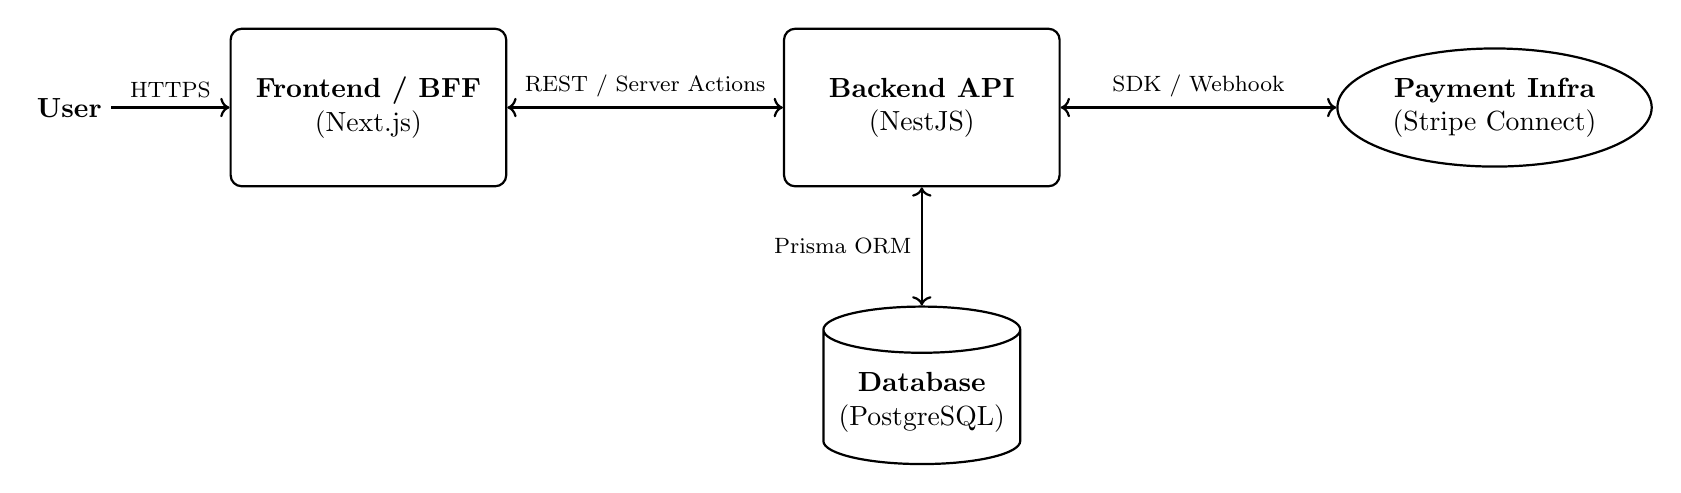
\begin{tikzpicture}[
				node distance=1.5cm and 3.5cm,
				box/.style={draw, rectangle, rounded corners, align=center, minimum width=3.5cm, minimum height=2cm, fill=white, thick},
				db/.style={draw, cylinder, shape border rotate=90, aspect=0.25, align=center, minimum width=2.5cm, minimum height=2cm, fill=white, thick},
				cloud/.style={draw, ellipse, align=center, minimum width=3cm, minimum height=1.5cm, fill=white, thick},
				arrow/.style={-Latex, thick, <->},
				label_text/.style={font=\footnotesize, align=center}
			]
			% Nodes
			\node[box] (frontend) {\textbf{Frontend / BFF}\\(Next.js)};
			\node[box, right=of frontend] (backend) {\textbf{Backend API}\\(NestJS)};
			\node[db, below=of backend] (database) {\textbf{Database}\\(PostgreSQL)};
			\node[cloud, right=of backend] (stripe) {\textbf{Payment Infra}\\(Stripe Connect)};

			% Connections
			\draw[arrow] (frontend) -- node[midway, above, label_text] {REST / Server Actions} (backend);
			\draw[arrow] (backend) -- node[midway, left, label_text] {Prisma ORM} (database);
			\draw[arrow] (backend) -- node[midway, above, label_text] {SDK / Webhook} (stripe);

			% User Interaction
			\node[left=1.5cm of frontend] (user) {\textbf{User}};
			\draw[arrow, ->] (user) -- node[midway, above, label_text] {HTTPS} (frontend);

		\end{tikzpicture}
	}
	\caption{Payment Platform 2 のシステム構成}
	\label{fig:platform_architecture}
\end{figure}

\subsubsection{フロントエンド}
ユーザーとの接点となるフロントエンドには,Reactベースのフレームワークである Next.js (App Router) \cite{nextjs} を採用した.本システムでは,単なる画面描画だけでなく,サーバーサイドでのデータフェッチや認証セッション管理を行うBFFとしての役割も担わせている.

\paragraph{ディレクトリベース・ルーティングの採用}
ソースコード構成(src/app配下)において,ファイルシステムの階層構造をそのままURLパスにマッピングするディレクトリベース・ルーティングを採用した.
例えば,クリエイターのポートフォリオページは src/app/[userPubId]/page.tsx,作品詳細ページは src/app/[userPubId]/[itemPubId]/page.tsx として配置されている.このように動的パラメータをディレクトリ名に含めることで,https://domain.com/user123/item456 のような,直感的で可読性の高いURL構造を容易に実現している.

\paragraph{Server Actionsとデータ取得の最適化}
コンポーネント設計においては,React Server Components (RSC) を全面的に採用した.作品情報(Markdownテキスト)やユーザープロファイルなどの静的な初期データは,サーバーサイドでデータベース(またはバックエンドAPI)から直接取得し,HTMLとしてクライアントに送信される.
また,フォーム送信や入札アクションなどの動的な操作には Server Actions (src/actions/) を用いることで,クライアントサイドに露出するAPIエンドポイントを隠蔽しつつ,型安全な関数呼び出しとしてバックエンドとの通信を実装している.

\paragraph{ 認証と認可}
認証基盤には Node.jsのライブラリであるNextAuth.js (src/api/auth/[...nextauth]) を導入し,Google OAuthおよびメールアドレス認証によるセキュアなログインフローを構築した.セッション情報はJWT(JSON Web Token)として暗号化され,HTTP Only Cookieを用いて管理される.

\subsubsection{バックエンド}
システムのコアロジックを担当するバックエンドには,Node.jsフレームワークである NestJS \cite{nestjs} を採用した.このフレームワークは、複雑なCtoC取引のステート管理や,金銭に関わる厳密なバリデーションを行うため,TypeScriptによる静的型付けと,依存性の注入(DI)によるモジュラーアーキテクチャを徹底している.

\paragraph{モジュール分割による関心の分離}
アプリケーションは機能単位でモジュールに分割されている.
\begin{description}
	\item[User Module] アカウント管理,プロフィール更新
	\item[Auth Module] 認証処理
	\item[Item Module] 作品のCRUD,Markdown解析,在庫管理
	\item[Order Module] 注文作成,決済ステータスの遷移管理
	\item[Project Module] 企画のガバナンス管理,収益分配計算
\end{description}
このようにドメインごとに責務を分離することで,コードの可読性を高めるとともに,特定の機能(例:オークション処理)に変更が生じた際の影響範囲を最小限に抑えている.

\paragraph{非同期イベント処理}
本システムでは決済処理をStripeに委譲しているため,決済の成功・失敗や,オークションにおける与信枠の確保の結果は,すべて非同期のWebhookイベントとして通知される.
これを受け取るための専用のエンドポイント (src/webhook) を実装し,Stripeからの署名検証を行った上で,Order データベースのステータスを安全に更新する仕組みを構築した.これにより,ネットワーク遅延や一時的な障害が発生しても,最終的なデータの整合性が保証される.

\subsubsection{データベース}
データの永続化には,リレーショナルデータベースである PostgreSQL \cite{postgresql} を採用した.複雑な多対多のリレーション(例:ProjectとCollaborators,ItemとBids)を矛盾なく管理し,ACID特性(原子性,一貫性,独立性,永続性)を備えたトランザクション処理を実現するためである.

\paragraph{Prisma ORMによる型安全なデータアクセス}
アプリケーション層とデータベース層の架け橋として Prisma \cite{prisma} を使用している.schema.prisma ファイルに定義されたデータモデルに基づき,型定義ファイル(TypeScript型)が自動生成される.
これにより,バックエンドの開発において「存在しないカラムへのアクセス」や「型の不一致」といった単純なミスをコンパイル時に検出可能となり,開発効率と品質が大幅に向上した.

\paragraph{スキーマ駆動開発}
開発フローにおいては,まず schema.prisma でデータ構造(User, Item, Project等のモデル定義)を記述し,それを元にマイグレーション(prisma migrate)を実行してDBスキーマを更新する手法をとった.これにより,仕様書に定義されたデータモデルが,実装コードとデータベースの実体に乖離することなく,常に同期された状態を維持している.

\subsubsection{決済および送金基盤 (Stripe Connect)}
CtoCプラットフォームにおける金銭取引の要となる決済インフラには,Stripe Connect \cite{stripe} を採用した.本システムでは単なる決済代行だけでなく,売り手(クリエイター)への送金管理,本人確認,および複雑なオークション決済を実現するために,以下の高度な機能群を実装している.

\paragraph{連結アカウントによるユーザー管理}
プラットフォームに参加するクリエイター(売り手)は,Stripeの「連結アカウント」として管理される.User モデルの stripeAccountId カラムには,Stripe側で発行された一意のアカウントID(acct\_...)が保存される.
これにより,売上の入金先銀行口座の管理や,特定商取引法に基づく本人確認手続きといったセンシティブな業務をStripeの堅牢なインフラにオフロードしつつ,プラットフォームとしてのコンプライアンス遵守を実現している.

\paragraph{支払いと送金の分離}
資金フローにおいては,買い手からの支払いを即時に売り手へ送金するのではなく,「支払いと送金別方式」を採用した.
この方式では,買い手の決済は一度プラットフォームのアカウントに対して行われ,その後,任意のタイミングで売り手の連結アカウントへ送金が実行される.これにより,以下の要件を満たしている.
\begin{description}
	\item[エスクロー機能] 商品の発送完了や受け取り評価が行われるまで,プラットフォーム上で売上を一時的に保持し,トラブル時の返金を容易にする.
	\item[収益分配の柔軟性] プロジェクト主催者への手数料やプラットフォーム手数料を差し引いた上で,正確な金額をクリエイターに分配する.
\end{description}

\paragraph{オークションにおける与信枠の活用}
イングリッシュオークションや抽選販売において,最大の課題である「当選後の未払い」を防ぐため,クレジットカードの「オーソリゼーション」機能を活用した決済フローを構築した.
\begin{description}
	\item[与信枠確保]  入札や抽選応募の時点で,PaymentIntent を作成し,capture\_method: 'manual' オプションを用いてカードの与信枠のみを確保する.この段階では実際の請求は発生しない.
	\item[確定と解放]落札や当選が確定した時点で capture を実行し,売上を確定させる.一方,落選や高値更新が発生した場合は即座に cancel を実行し,与信枠を解放する.
\end{description}
この仕組みにより,ユーザーの資金拘束を必要最小限に抑えつつ,システム側は「支払い能力のある入札」のみを受け付けることが可能となり,取引の安全性を飛躍的に高めている.

\subsection{データモデル設計}
本システムのデータモデルは,User,Item,Project の3つのコアエンティティを中心に設計されている.主要なエンティティの関係性をfigure 1に示す.

\begin{figure}[t]
	\centering
	\begin{tikzpicture}[
			node distance=1.8cm,
			entity/.style={draw, rectangle, rounded corners, align=center, minimum width=2.5cm, minimum height=1.2cm, fill=white, thick},
			attribute/.style={draw, ellipse, align=center, minimum width=2cm, minimum height=0.8cm, fill=white},
			relationship/.style={draw, diamond, aspect=2, align=center, minimum width=2cm, minimum height=1cm, fill=white, thick},
			arrow/.style={-Latex, thick},
			line/.style={thick}
		]
		% Entities
		\node[entity] (user) {\textbf{User}};
		\node[entity, right=4cm of user] (item) {\textbf{Item}};
		\node[entity, below=3cm of user] (project) {\textbf{Project}};

		% Relationships
		% User - Item (Created By)
		\draw[arrow] (user) -- node[above] {作成 (1:N)} (item);

		% User - Project (Owner)
		\draw[arrow] (user) -- node[left] {所有 (1:N)} (project);

		% Project - Item (Contains)
		\draw[arrow] (project.east) -- node[right] {包含 (1:N)} (item.south);

		% User - Project (Collaborates)
		\draw[line, dashed] (user.south east) -- node[sloped, above, font=\footnotesize] {参加 (M:N)} (project.north east);

		% Attributes (Selected)
		\node[attribute, above left=0.5cm of user] (uid) {id, publicId};
		\node[attribute, left=0.5cm of user] (ustripe) {stripeAccountId};
		\draw[line] (user) -- (uid);
		\draw[line] (user) -- (ustripe);

		\node[attribute, above right=0.5cm of item] (iid) {id, price};
		\node[attribute, right=0.5cm of item] (inarrative) {description\\(Narrative)};
		\draw[line] (item) -- (iid);
		\draw[line] (item) -- (inarrative);

		\node[attribute, below left=0.5cm of project] (pid) {id, mode};
		\draw[line] (project) -- (pid);

	\end{tikzpicture}
	\caption{User, Item, Project のER図(主要なリレーションのみ抜粋)}
	\label{fig:er_diagram}
\end{figure}

\subsubsection{Userモデル}
User モデルは,本プラットフォームにおけるすべての活動の基点となる「主体」を表すリソースである.単なる認証用のアカウント情報とは異なり,インターネット上におけるクリエイターとしてのアイデンティティと,経済活動を行うための法的人格としての側面を併せ持つ.

\paragraph{公開識別子とポートフォリオ機能}
各ユーザーには,データベース内部の主キー(id)とは別に,外部公開用の識別子として publicId(CUID)が付与される.これにより,https://domain/[userPubId] という予測不可能な固有URLが生成される.このURLは,ユーザーの出品作品や参加プロジェクト,活動履歴を集約したポートフォリオページとして機能し,クリエイターのブランディングを支援する.

\paragraph{経済的主体としての属性}
CtoC取引における売り手としての機能を果たすため,Stripe ConnectのアカウントIDを stripeAccountId カラムに保持する.これは,本人確認が完了したユーザーにのみ発行されるIDであり,このフィールドの有無によって,システムはユーザーが「出品可能」か「購入専用」かを判別する.また,買い手としての情報は stripeCustomerId に紐づけられ,クレジットカード情報等の機微な決済情報はすべてStripe側のVaultに保存される設計としている.

\paragraph{多層的なリレーション}
Userは他のリソースと多層的な関係を持つ.自身が作成した作品(items)だけでなく,他者と共同制作した作品(contributingItems)や,主催する企画(ownedProjects),参加者として関わる企画(contributingProjects)へのリレーションを保持し,個人の活動の広がりをグラフ構造として表現する.

\subsubsection{Itemモデル}
Item モデルは,取引の対象となる「作品」を管理するリソースである.既存のECサイトにおける「商品」モデルと決定的に異なる点は,物理的なスペック情報よりも「ナラティブ」の記述と保存に重きを置いている点である.

\paragraph{ナラティブの保存}
作品の背景ストーリーや制作過程を記録するために,description フィールドにはMarkdown形式のテキストデータが保存される.フロントエンド側ではこれがリッチテキストとしてレンダリングされ,画像や動画の埋め込みとともに,作品単体で完結した「記事」として表示される.これにより,物理的な展示会場においてQRコード経由でアクセスされた際,鑑賞者に深い理解を促すキャプションボードとしての役割を果たす.

\paragraph{販売ロジックの抽象化}
一点物や限定品など,作品の性質に応じた最適な販売形態を選択可能にするため,salesMethod カラム(ENUM型)を定義している.
\begin{description}
	\item[AUCTION] イングリッシュオークション形式.currentPrice や endTime と連動し,入札を受け付ける.
	\item[LOTTERY] 抽選販売形式.事前与信を用いた応募ロジックが適用される.
	\item[FIXED\_PRICE] 定額販売形式.即時購入が可能となる.
\end{description}

\paragraph{ステータス管理}
作品のライフサイクルを管理するために,status カラム(ENUM型)を用いる.出品前の DRAFT,販売中の FOR\_SALE,取引成立後の SOLD などの状態遷移を厳密に定義することで,不正な購入や二重決済を防ぐ排他制御を実現している.また,Stripeの商品マスタと同期するために stripeProductId および stripePriceId を保持し,決済システムとの整合性を保っている.

\subsubsection{Projectモデル}
Project モデルは,複数の User と Item を束ねる「共同体」および「文脈」を提供するリソースである.これは単なるカテゴリ分類タグではなく,独自の経済圏を持つ「企画」そのものをデジタル上に実体化させたものである.

\paragraph{ガバナンス構造の表現}
\begin{description}
	\item[Owner] プロジェクトの作成者であり,管理者権限を持つ.ownerId 外部キーによってUserモデルと一対多で結ばれる.
	\item[Collaborators] 企画に参加するクリエイター群.中間テーブルを介した多対多のリレーションによって定義される.
	      この構造により,招待制のサークル活動や,主催者が権限を持つコンテストなど,多様な組織形態をシステム上で再現可能にしている.
\end{description}

\paragraph{経済圏としての機能}
Projectは,紐づけられた作品群(items)の集合体として機能する.Item モデルは projectId を外部キーとして持ち,自身がどの文脈に属しているかを示す.このリレーションに基づき,システムは「企画単位での売上集計」や「主催者への手数料分配」といった高度な金銭処理を実行する.すなわち,Projectモデルは単なるグルーピング機能ではなく,収益分配の計算単位としても機能する設計となっている.

\subsection{Project管理方式}
本プラットフォームにおける Project は,単なる商品カテゴリや検索タグではなく,独自の規律と経済ルールを持つ「共同体」として定義される.
現実世界の創作活動には,大学のサークル活動のような水平的な人間関係に基づくものから,コンテストのように主催者が強い権限を持つ垂直的な構造,あるいはインターネット上のミームのように不特定多数が自律的に参加するものまで,多種多様な形態が存在する.
これらを単一のシステム仕様でカバーすることは困難であるため,本システムでは Project リソースに対して3つの異なるガバナンスモード(管理方式)を実装した.

\subsubsection{Cooperative Mode}
\paragraph{意義と適用領域}
Cooperative Mode は,既知のメンバー間の「信頼」を基盤とした小規模から中規模の共同体を再現するためのモードである.大学のサークル活動,グループ展,あるいは特定のクリエイター同士のコラボレーション企画などを想定している.ここでは,厳格な管理コストを削減し,メンバー間の自律的な調整を優先する運用がなされる.


\paragraph{仕様詳細}
\begin{description}
	\item[参加権限] 「招待制」を採用する.プロジェクトオーナーまたは既存メンバーからの招待リンク(署名付きURL)を受け取ったユーザーのみが,Collaboratorとして参加できる.
	\item[作品管理] 参加メンバーは,自身の判断で作品(Item)をProjectに紐づけ,即座に公開することができる.オーナーによる事前承認プロセスは存在しない.
	\item[収益構造] 原則として,売上は各作品の制作者に直接帰属する.オーナーによる「場所代」の強制徴収機能は無効化されており,金銭的な搾取が発生しない構造となる。
\end{description}

\subsubsection{Managed Mode}
\paragraph{意義と適用領域}
Managed Mode は,明確な主催者が存在し,品質管理やレギュレーションの遵守が求められる階層型の共同体である.企業主催のコンテスト,有名インフルエンサーによる企画展,アンソロジーの編纂などを想定している.
このモードの核心は,主催者に対して「管理権限」と引き換えに「経済的インセンティブ」を与える点にある.これにより,従来はボランティアに依存していた企画運営業務(キュレーション,広報,進行管理)を,収益を生む事業として成立させることを可能にする.

\paragraph{仕様詳細}
\begin{description}
	\item[参加権限] 「公募制」を採用する.ユーザーはProjectに対して参加申請を行い,オーナーが管理画面でこれを「承認」または「拒否」することでメンバーシップが確定する.
	\item[作品管理] 出品された作品は一時的に PENDING ステータスとなり,オーナーが内容を確認し承認するまで公開されない.また,オーナーは規約違反の作品を強制的にプロジェクトから除外する権限を持つ.
	\item[収益構造] Stripe Connectの "Separate Charges and Transfers" APIを活用し,「主催者手数料」 の設定を可能にしている.取引成立時,システムは売上総額からプラットフォーム手数料と主催者手数料を自動的に控除し,残額を作品制作者へ送金する.
\end{description}

\subsubsection{Theme Mode}
\paragraph{意義と適用領域}
Theme Mode は,中央集権的な管理者を排し,共通の文脈やテーマの下に不特定多数の主体が自律的に集合する「創発的な共同体」である.インターネット上で突発的に発生するトレンドや,特定のハッシュタグを介して形成される大規模な社会現象,あるいは季節的なイベントに伴う集合知的な制作活動をモデル化している.
本モードの設計目的は,参加における許認可プロセスを完全に撤廃することで参入障壁を最小化し,ネットワーク外部性を最大限に作用させることにある.これにより,短期間で幾何級数的な作品数の増加とトラフィックの凝集を実現する.

\paragraph{仕様詳細}
\begin{description}
	\item[参加権限] 「自由参加」を採用する.アカウントを持つ全ユーザーは,許可を得ることなく即座にProjectに参加できる.
	\item[作品管理] 紐づけられた作品は即時公開される.オーナー(発起人)は,通報対応を除き,他者の作品を削除する権限を持たない.
	\item[収益構造] 主催者手数料の設定は不可である.売上はすべて作品制作者に還元される.これにより,発起人が「他人の作品で金儲けをしている」という批判を避けることができ,純粋なムーブメントとしての成長を促進する.
\end{description}

\subsubsection{Project 管理方式の比較}
各モードにおける権限と金銭的フローの差異を示す。
\begin{table}[h]
	\caption{インダストリアルアートの授業}
	\label{tab:sample}
	\centering
	\begin{tabular}{lccccc} % l:Left, c:Center, r:Right 寄せ
		\hline
		方式名         & 参加フロー       & 作品公開フロー     & 主催者権限    & 収益分配(Organizer Fee) \\
		\hline \hline
		Cooperative & 招待のみ        & 即時公開        & メンバー除名可  & 不可                  \\
		Managed     & 申請 $\to$ 承認 & 投稿 $\to$ 承認 & 作品削除・否認可 & 可                   \\
		Theme       & 自由参加        & 即時公開        & 管理不可     & 不可                  \\
		\hline
	\end{tabular}
\end{table}

\subsection{統合型検索システム}
本プラットフォームにおける検索機能は,単に特定の物品を発見するためのツールではなく,ユーザーを未知の作品やクリエイター,あるいはコミュニティへと導く「ディスカバリー」の中核機能として位置づけられる.
ユーザーの探索意図は,「特定の作品が欲しい」だけでなく,「面白い企画はないか」や「特定の作家の活動を知りたい」など多岐にわたる.これら多様な検索意図を単一のインターフェースで充足させるため,User,Item,Project の3つの主要リソースを横断的に検索する「統合型オムニサーチシステム」を実装した.

\subsubsection{設計思想: 探索的検索への対応}
従来のEコマースサイトにおける検索システムは,SKU(最小管理単位)ベースの商品検索に特化しており,ユーザーが明確な購買目的を持っていることを前提とすることが多い.
しかし,一点物や創作活動を扱う本プラットフォームにおいては,ユーザーは必ずしも具体的な商品名を検索するとは限らない.「折り紙」「ガレージキット」といったジャンル名や,「学園祭」といったイベント名から検索を開始し,そこから関連するクリエイターや作品群へと興味を広げていく「探索的検索」の行動様式が支配的である.
したがって,検索システムは,単一のリソースリストを返すのではなく,システム内の多様なエンティティ(主体,文脈,作品)を網羅的に提示し,ユーザーの回遊を促す情報アーキテクチャを持つ必要がある.

\subsubsection{アーキテクチャ: 並列クエリ実行モデル}
オムニサーチのバックエンド処理においては,異なるデータ構造を持つ複数のテーブルに対する検索を効率的に処理するため,並列クエリ実行モデルを採用した.
具体的には,ユーザーが入力した単一の検索クエリに対し,バックエンド(NestJS)は以下の処理を非同期かつ並列に実行する.
\begin{description}
	\item[Project Search] プロジェクト名および概要文に対する全文検索またはベクトル検索.
	\item[User Search] ユーザー名およびプロフィール文に対する検索.
	\item[Item Search] 作品名,説明文(Markdown),タグに対する検索.
\end{description}
これらのクエリは Promise.all 等を用いて並行してデータベース(PostgreSQL)に発行され,個別の検索結果が得られ次第,単一のレスポンスオブジェクトに統合されてクライアントへ返却される.これにより,リソースごとに個別の検索画面を遷移する必要をなくし,シームレスな検索体験を実現している.

\subsubsection{インターフェース: 階層的情報の統合表示}
検索結果の表示画面においては,情報の重要度とユーザーの認知負荷を考慮し,リソースタイプごとに優先順位を設けた階層的表示を採用した.
\begin{description}
	\item[上部: 関連プロジェクト] 検索結果の最上部には,クエリに関連性の高い Project を最大3件表示する.これは,個別の作品よりも「企画」や「イベント」という大きな文脈を優先して提示することで,ユーザーをコミュニティ全体へと誘導するためである.
	\item[中部: 関連クリエイター] 次に,関連する User を最大5件表示する.これにより,特定の作家を探しているユーザーのナビゲーション意図に即座に応える.
	\item[下部: 関連作品] 最下部には,関連する Item をグリッド形式で表示する.ここでは無限スクロールを採用し,ユーザーが満足するまで作品を閲覧し続けられるよう設計している.
\end{description}
また,検索結果画面のサイドバーには,「ファセットナビゲーション」を配置した.ユーザーは,統合検索によって得られた広範な結果から,価格帯,カテゴリ,販売方式(オークション・定額など)といった属性に基づいて動的に絞り込みを行うことができる.これにより,探索的な「広げる検索」と,条件を特定する「絞る検索」の両立を図っている.

\subsection{販売形態と価格決定アルゴリズム}
本プラットフォームが扱う「一点物」や「希少在庫」の流通において,固定価格での販売は必ずしも最適解ではない.需要が供給を大幅に上回る場合,価格メカニズムが機能せず「早い者勝ち」となることで,適正価格の販売ではなくなるからである.
この課題を解決し,作品を最も必要とするユーザーへ適正価格で配分するために,本システムでは以下の4つの販売アルゴリズムを実装した.また,全ての方式において,Stripe Connect APIを用いたクレジットカードの与信枠確保を必須とすることで,CtoC取引における最大の問題である支払い不履行を低減している。

\subsubsection{イングリッシュ・オークション}
在庫が単一($N=1$)である一点物の作品に対し,最も高い評価額を持つ購入希望者を決定するための標準的な競り上げ方式である.

\paragraph{自動入札アルゴリズム}
ユーザーの利便性とサーバー負荷の軽減を考慮し,Vickrey Auctionの概念を取り入れた自動入札システムを採用した.
ユーザーは「現在価格」ではなく,自身の「支払ってもよい最高額」を入力する.システムは,2番目に高い入札額(または開始価格)に最小入札単位を加えた額を「現在価格」として自動的に算出・更新する.これにより,ユーザーは画面に張り付いて再入札を繰り返す必要がなくなり,合理的な入札行動が促進される.

\paragraph{連続的な与信枠管理フロー}
本システムでは,「最高入札者は常に支払い能力を保証されている」という状態を維持するため,最高入札者が入れ替わるたびに決済リソースの「ハンドオーバー」を行う.具体的なトランザクションフローは以下の通りである.
\begin{description}
	\item[1. 新規与信] 新たな高値入札者が現れた際,システムはそのユーザーのクレジットカードに対し,入札額全額の与信枠確保(paymentIntents.create with capture\_method: 'manual')を試行する.これに失敗した場合,入札自体を却下する.
	\item[2. DB更新] 与信確保に成功した場合のみ,データベース上の Item レコード(現在価格,リーダーID)および Bid レコードを更新する.
	\item[3. 旧与信解放] 更新完了後,直前の最高入札者の与信枠(PaymentIntent)に対してキャンセル処理(paymentIntents.cancel)を非同期的に実行し,枠を即時解放する.
\end{description}
このプロセスにより,オークション終了時に「落札者が支払えない」というリスクを回避している。

\subsubsection{複数点式オークション}
在庫が複数($N > 1$)存在するが,需要がそれを上回る場合(例:限定5個のガレージキット)に適用される,本システム独自の販売方式である.従来の単一価格オークションではなく,入札額がそのまま支払額となる Pay-as-Bid方式 を採用した.
\paragraph{当選者決定ロジック}
入札額の高い順にソートを行い,上位 $N$ 名を当選者として確定する.
\[
	B_{1} \ge B_{2} \ge \dots \ge B_{N} \ge \dots \ge B_{M}
\]
ここで $B_{i}$ は $i$ 番目のユーザーの入札額であり,上位 $N$ 名までの入札が有効となる.同額入札が存在する場合は,先着優先として順位付けを行う.
\paragraph{Pay-as-Bidによる収益最大化}
当選者全員が $B_{N}$(ボーダーライン価格)を支払う単一価格方式ではなく,各当選者が自身の提示した $B_{i}$ を支払う Pay-as-Bid 方式を採用した.
これにより,作品に対し強い選好を持つ熱狂的なファン($B_{1}$)からは高い収益を,学生などの価格に敏感な層($B_{N}$)からは適正な収益を得ることが可能となる.結果として,同一の商品であっても購入者の支払意思額に応じた価格差別化が自然発生し,クリエイターへの還元額を最大化する.
\paragraph{取引および決済フローの詳細}
本方式では,複数の当選候補者が並存するため,イングリッシュ・オークションのような「入れ替え」ではなく「全件確保」に近い戦略をとる.
\begin{description}
	\item[Step 1: 入札と与信確保 ] ユーザーが入札を行う際,システムは即座に入札額全額の与信枠確保を実行する.この時点で決済は確定しないが,カードの利用枠は押さえられる.これにより,冷やかしや入札後の支払い拒否を未然に防ぐ.
	\item[Step 2: ボーダーラインの可視化と競争] オークション期間中,入札画面には「現在,上位 $N$ 位に入るための最低価格($B_{N}$)」がリアルタイムで表示される.ユーザーはこのボーダーラインを参考に,自身の予算内で入札額を調整する.
	\item[Step 3: 決着と一括決済] 決着と一括決済 (Settlement)終了時刻(endTime)に到達した時点で,システムは全入札を確定させる.
	      上位 $N$ 名: 確保していた与信枠に対し capture を実行し,売上を確定させる.
	      落選者 ($N+1$ 位以下): 確保していた与信枠に対し cancel (Void) を実行し,即座に解放する.
\end{description}
\subsubsection{抽選販売}
価格の高騰を抑制したい場合や,機会の平等を重視する場合に用いられる方式である.技術的な特異点は,応募プロセスにおける事前与信の導入にある.
\paragraph{フローとステート管理}
\begin{description}
	\item[応募時] ユーザーが「応募」ボタンを押下した瞬間に,商品価格分の与信枠確保を実行する.確保に失敗した場合,応募は受理されない.
	\item[抽選時] 擬似乱数生成器を用いて当選者を選出する.
	\item[確定時] 当選者の取引ステータスを CAPTURED に更新し,決済を確定させる.同時に,落選者に対しては VOID 処理を行い,与信枠を即時解放する.
\end{description}
この仕組みにより,従来のアナログな抽選販売で頻発していた「当選連絡後の音信不通」や「支払い拒否」による再抽選の手間を完全にゼロにし,運用コストを最小化している.

\subsubsection{定額販売}
在庫が無制限,あるいは需給バランスが安定している作品向けの,一般的なECと同様の販売方式である.即時決済(Capture)によって取引が成立する.

\subsection{テストデータに対する要件と課題}
このような「文脈重視型」かつ「複雑なリレーションを持つ」プラットフォームの開発において,テストデータの用意は大きな課題であった.

\begin{enumerate}
	\item \textbf{リレーションの整合性}:
	      ランダムなデータを生成すると,「ユーザーが未参加のプロジェクトに関連する作品を出品している」といった外部キー制約違反や論理矛盾が頻発する.これを防ぐためには,データベースの依存関係を深く理解した生成ロジックが必要となる.

	\item \textbf{コンテンツのリアリティ}:
	      UIの検証(例えば,長い説明文がレイアウト崩れを起こさないか,検索機能が適切にキーワードを拾うか)を行うためには,「Lorem Ipsum」に代表される無意味なダミーテキストではなく,ドメイン固有の用語や適切な長さを持つ「リアルなテキスト」が必要である.特に本プラットフォームでは「制作ログ」や「物語」が主要なコンテンツであるため,その質がUX評価に直結する.

	\item \textbf{多様性の確保}:
	      検索アルゴリズムやレコメンデーション機能の性能を評価するためには,データの分布に偏りがあってはならない.特定のカテゴリ(例:アクセサリー)だけにデータが集中すると,システムの性能を正しく評価できない.
\end{enumerate}

第3章で提案したデータ生成エージェントは,これらの課題,特に「整合性」と「多様性」の両立という課題を解決するために設計されたものであり,本プラットフォームはその有効性を検証するための最適なテストベッドであると言える.

\section{評価実験}
\label{chap:evaluation}

本章では,提案手法である「RAGを用いたデータ生成エージェント」の有効性を検証するために実施した比較実験の結果について述べる.
本実験では,過去の生成履歴を参照する記憶機構(RAG)の導入が,生成される社会的シナリオの多様性と品質に与える影響を評価する.具体的には,RAGにより類似内容の重複生成(モード崩壊)の発生が抑制されるか,および生成品質が維持されるかを,定量評価と定性評価の両面から検証する.

\subsection{実験設定}
以下の条件において,それぞれ1000件のシナリオデータ(User-Project-Itemのセット)を連続生成し,評価用データセットとした.
本実験の目的は,RAGの有無による差を比較可能にすることであり,(1) 語彙的多様性,(2) ベクトル類似度に基づく重複度合い,(3) LLM as a Jadgeによる定性評価,(4)高類似度,低類似度ペアのシナリオ・実データの定性評価の四つの観点から評価を行った.

\begin{table}[h]
	\centering
	\caption{実験条件とパラメータ}
	\label{tab:conditions}
	\begin{tabular}{l|l|l|c}
		\hline
		実験ID         & 基盤モデル (LLM)    & RAG (メモリ参照) & データ数 \\
		\hline \hline
		\textbf{A-1} & Gemini 3 Pro   & \textbf{ON} & 1000 \\
		\textbf{A-2} & Gemini 3 Pro   & OFF         & 1000 \\
		\textbf{B-1} & Gemini 3 Flash & \textbf{ON} & 1000 \\
		\textbf{B-2} & Gemini 3 Flash & OFF         & 1000 \\
		\textbf{C-1} & GPT-5.2        & \textbf{ON} & 1000 \\
		\textbf{C-2} & GPT-5.2        & OFF         & 1000 \\
		\textbf{D-1} & GPT-5 Mini     & \textbf{ON} & 1000 \\
		\textbf{D-2} & GPT-5 Mini     & OFF         & 1000 \\
		\hline
	\end{tabular}
\end{table}

すべての条件において,生成カテゴリは \texttt{PLASTIC\_MODEL}, \texttt{HANDCRAFT}, \texttt{GADGET} の3つを均等に生成するよう指示し,生成の多様性を確保するためにTemperatureパラメータは \texttt{0.9} に設定した.
なお,本節でいう生成カテゴリ(\texttt{PLASTIC\_MODEL}等)は,エージェントのDirectorノードで定義されたタスク属性であり,生成するシナリオクラスターがどのジャンルの出品(Item)に対応するかを示すラベルである.Directorは,目標分布(\texttt{targetDistribution})に基づいて次に生成すべきカテゴリを選択し,カテゴリごとに定義された分布マトリクス(\texttt{DISTRIBUTION\_MATRIX})に従って構造タイプ(\texttt{structureType})をサンプリングし,その組を生成タスクとして下流ノードへ渡す(\texttt{agent/src/nodes/director.ts}).

\subsection{生成データの実例}
本実験により生成されたデータの一例として,「夜間大学・無線同好会」というテーマに基づいたシナリオをコードリスト\ref{lst:generated_example}に示す.
この例では,3名のユーザー(霧島えみ,矢木拓真,水瀬ナオ)と,彼らが共有するプロジェクト(都市電波ノイズ可視化マップ),および制作された作品(Item)が生成されている.
本研究で想定する最小生成単位(User-Project-Itemのセット)として,(1) 複数ユーザーが同一Projectに紐づき,(2) 各Itemが作成者(\texttt{authorId})に対応し,(3) テキスト記述が活動の背景や判断基準を含む,という前提が満たされているかを確認するため,本節で例示する.

\lstinputlisting[
  caption={生成されたシナリオデータの例(夜間大学・無線同好会)},
  label={lst:generated_example},
  language=json
]{example-data.jsonc}
コードリスト\ref{lst:generated_example}は,実験データ(\texttt{data.jsonl})から抽出した1レコードを整形したものである.レコードは実験メタデータ(\texttt{runId}, \texttt{generatedAt}),シナリオの要約(\texttt{scenario}),および生成されたデータ本体(\texttt{cluster})から構成される.\texttt{cluster} 内には,ユーザー集合(\texttt{users})および企画・成果物に相当するデータが含まれており,各要素は \texttt{tempId} により参照可能である.また,\texttt{bio} や \texttt{description} には,活動の背景や判断基準(例:法規・運用上の前提,制作上の意図)が記述されており,社会的シナリオとしての文脈が含まれている.

Scenarist Agentの前提および制約は,コードリスト\ref{lst:prompt_scenarist}に示すシステムプロンプトに記述されている.同プロンプトでは,webシステムがCtoCの創作・ホビー・コレクションのプラットフォームであること,Itemが個人が売買・展示可能な範囲の対象であること,およびカテゴリが\texttt{PLASTIC\_MODEL}の場合に「本物の兵器ではない」こと等を前提としている.また,\texttt{tempId} によるリレーション構築,\texttt{publicId} の命名制約,およびMarkdown形式の説明文等が制約として与えられている.
コードリスト\ref{lst:generated_example}ではカテゴリが\texttt{GADGET}であり,成果物は自作アンテナや可視化UI設定等の出品として記述されている.これはプロンプトが定める「個人が売買・展示可能な対象」という前提に沿う.また,各要素に \texttt{tempId} と \texttt{publicId} が付与され,\texttt{ownerId} や \texttt{authorId},\texttt{projectId} 等を通じた参照関係も含まれていることから,プロンプトが要求するリレーション構築および命名制約が反映されていることが確認できる.さらに,\texttt{description} にはMarkdown形式の記述が含まれており,説明文に一定の長さと具体性が付与されている.

\subsection{語彙数の増加推移}
生成されたデータセットの語彙的多様性を測る指標として,テキストに含まれる「ユニーク単語数」の増加推移を解析した.類似した表現が繰り返される場合,生成数の増加に伴って新出語彙の増加が鈍化する可能性があるため,本節では累積ユニーク数の推移を比較する.

\subsubsection{解析手法}
各シナリオの \texttt{theme} フィールドを対象に分かち書きを行い,累積ユニーク単語数をカウントした.分かち書きおよび集計は,実験用スクリプト(\texttt{agent/scripts/experiment/analysis/vocabulary/analyze\_vocabulary.ts})に従い,\texttt{Intl.Segmenter}(locale: \texttt{ja}, granularity: \texttt{word})でセグメントに分割した後,\texttt{isWordLike} が真となるセグメントを単語として採用した.また,\texttt{isWordLike} が偽であっても,文字または数字のみからなるセグメントは単語として採用した.各単語は小文字化した上で集合に追加し,生成順に集合サイズを記録することで,生成ステップごとの累積ユニーク数を算出した.

\subsubsection{結果と考察}
図\ref{fig:vocabulary_growth}に,生成ステップ数に伴う語彙数の増加推移を示す.

\begin{figure}[h]
	\centering
	\includegraphics[width=0.9\textwidth]{figure/vocabulary_growth_comparison.png}
	\caption{生成数に伴うユニーク語彙数の増加推移}
	\label{fig:vocabulary_growth}
\end{figure}

実験の結果,1000件生成時点での総語彙数は以下の通りとなった.

\begin{itemize}
	\item \textbf{GPT-5.2}: RAG ONで4,425語に対し,OFFでは3,368語 (\textbf{+31.4\%})
	\item \textbf{Gemini 3 Flash}: RAG ONで3,041語に対し,OFFでは2,187語 (\textbf{+39.0\%})
\end{itemize}

すべてのモデルにおいて,RAGを有効にした場合の方が,より多くの語彙が観測された.特に増加の推移に注目すると,RAG OFF群(図中暖色系)では後半に増加が鈍化する傾向が見られる一方,RAG ON群(図中寒色系)では増加が継続している.
この結果は,本実験の条件下では,記憶機構により過去の生成物との差別化が促され,新しい語彙が導入されやすくなる可能性を示唆する.

\subsection{ベクトル類似度による重複検知}
次に,生成されたデータ同士がどの程度似通っているかを評価し,RAGの有無によって重複度合いがどのように変化するかを検証した.本節の目的は,個別のテーマ文だけでなく,シナリオ全体(Theme, User, Project, Item)を含む記述の類似性をベクトル空間上で定量化することである.

\subsubsection{解析手法}
各シナリオに含まれるすべてのエンティティ(Theme, User, Project, Item)のテキストプロパティ(名前,説明文,属性など)を連結し,単一の文字列としてEmbeddingモデル(\texttt{gemini-embedding-001})によりベクトル化した.これにより,単なるあらすじだけでなく,詳細な設定レベルでの類似性を評価した.
その後,生成された全ペア($_{1000}C_2$ 通り)のコサイン類似度分布を計算し,RAGの有無による効果量(Cohen's $d$)を算出した.

\subsubsection{結果と考察}
図\ref{fig:similarity_histogram}にコサイン類似度の分布を示す.
また,表\ref{tab:similarity_stats}に各モデルにおける類似度の変化と効果量を示す.

\begin{figure}[h]
	\centering
	\includegraphics[width=0.9\textwidth]{figure/similarity_distribution_grid_v2.png}
	\caption{生成データ間のコサイン類似度分布(全プロパティ結合Embedding)}
	\label{fig:similarity_histogram}
\end{figure}

\begin{table}[h]
	\centering
	\caption{RAG有無による平均類似度の変化と効果量}
	\label{tab:similarity_stats}
	\begin{tabular}{l|c|c|c}
		\hline
		モデル                     & 平均類似度 (OFF $\to$ ON) & 差分              & Cohen's $d$    \\
		\hline \hline
		\textbf{GPT-5.2}        & 0.806 $\to$ 0.785    & \textbf{-0.021} & \textbf{-0.51} \\
		\textbf{GPT-5 Mini}     & 0.802 $\to$ 0.786    & -0.016          & -0.40          \\
		\textbf{Gemini 3 Flash} & 0.783 $\to$ 0.767    & -0.016          & -0.39          \\
		\textbf{Gemini 3 Pro}   & 0.771 $\to$ 0.770    & -0.001          & -0.01          \\
		\hline
	\end{tabular}
\end{table}

% 平均類似度の比較結果は以下の通りである(低いほど多様性が高い).

実験の結果,Gemini 3 Proを除くすべてのモデルにおいて,RAGを有効にすることで類似度の分布が低い側へ移動する傾向が見られた.
特にGPT-5.2においては,効果量 $d=-0.51$ が得られており,RAG ON条件で平均類似度が低下している(表\ref{tab:similarity_stats}).
Gemini 3 Proにおいて差分が小さい点については,本実験の条件下ではOFFとONで平均類似度が近く,RAGによる変化が相対的に小さかった可能性がある.

\subsection{LLM Judgeによる定性評価}
多様性の向上が品質(整合性や具体性等)の低下を伴わないかを確認するため,Gemini 3 Proを用いた定性評価を実施した.各条件から20件ずつランダムに抽出したシナリオに対し,評価用LLMが以下の3観点で評価を行った(以降,LLM Judgeと表記する).

\subsubsection{評価基準}
各シナリオに対し,以下の3つの観点を5段階でスコアリングした.
\begin{enumerate}
	\item \textbf{整合性}: 設定の矛盾がないか.
	\item \textbf{具体性}: 固有名詞,数値,専門用語が含まれているか.
	\item \textbf{人間らしさ}: AI特有の機械的な記述ではなく,熱量や生活感があるか.
\end{enumerate}

\subsubsection{結果概要}
全4モデルにおけるRAGの有無によるスコア比較を表\ref{tab:judge_results}に示す.

\begin{table}[h]
	\centering
	\caption{LLM Judgeによる定性評価結果(各条件20件抽出,5段階評価)}
	\label{tab:judge_results}
	\begin{tabular}{l|c|c|c|c}
		\hline
		モデル                     & 条件          & 整合性 (Coherence) & 具体性 (Specificity) & 人間らしさ (Human-like) \\
		\hline \hline
		\textbf{GPT-5 Mini}     & OFF         & 5.00            & 4.75              & 4.15               \\
		                        & \textbf{ON} & \textbf{5.00}   & \textbf{4.95}     & \textbf{4.30}      \\
		\hline
		\textbf{Gemini 3 Flash} & OFF         & 5.00            & 5.00              & 4.75               \\
		                        & \textbf{ON} & \textbf{5.00}   & \textbf{5.00}     & \textbf{4.95}      \\
		\hline
		\textbf{GPT-5.2}        & OFF         & 5.00            & 5.00              & 5.00               \\
		                        & ON          & 5.00            & 5.00              & 4.95               \\
		\hline
		\textbf{Gemini 3 Pro}   & OFF         & 5.00            & 5.00              & 5.00               \\
		                        & ON          & 4.95            & 5.00              & 5.00               \\
		\hline
	\end{tabular}
\end{table}

結果として,すべてのモデルにおいて「整合性」は高いスコアを記録した(表\ref{tab:judge_results}).また,「具体性」や「人間らしさ」についても,本実験のサンプルでは条件間で大きな差は観測されなかった.

\subsubsection{定性的考察:具体性と専門性}
生成されたシナリオの内容を確認すると,RAGの有無にかかわらず,専門用語や制作上の判断基準が記述されている事例が見られた.以下に,LLM Judgeによって抽出された事例を示す.

\begin{description}
	\item[事例1: 専門的具体性の向上] \mbox{} \\
	      \textbf{テーマ}: 自然風化・天然ウェザリング至上主義「プラスチック盆栽」学会 \\
	      \textbf{評価コメント}: 「具体的なキット名(RGザク、サザビーVer.Ka)、設置環境(室外機の上)、劣化メカニズム(加水分解、紫外線退色)が極めて詳細かつ論理的に描写されています。塗装=欺瞞という独自の哲学にも熱量を感じます。」

	\item[事例2: 独自の視点と人間らしさ] \mbox{} \\
	      \textbf{テーマ}: 巨大人型兵器の足元にある「都市インフラ」景観保存委員会 \\
	      \textbf{評価コメント}: 「『ロボット本体には関心がない』という特異なテーマが一貫しており、0.2mm真鍮線や座屈、応力集中といった専門用語が多用され解像度が高い。AI特有の不自然さを感じさせない,強いこだわりが反映された内容である.」

	\item[事例3: 現代的な風刺とユーモア] \mbox{} \\
	      \textbf{テーマ}: デジタル世界の『不快なUI』を物理ガジェットとして再現する \\
	      \textbf{評価コメント}: 「Cookie同意バナーやreCAPTCHAといったデジタルストレスを物理化するという発想が秀逸。『トロールの快感』といったブラックユーモアを含む記述には、AI生成とは思えない強い人間味が感じられます。」
\end{description}

本実験の範囲では,RAGの導入は定性評価スコアに大きな変化を与えない結果となった.

\subsection{数値的類似度と意味的多様性の関係}
前節までの評価により,RAGの導入がコサイン類似度を低下させ,語彙数を増加させることが確認された.しかし,Embeddingの数値的な類似度が低いことが,必ずしも「人間にとって意味のある多様性」につながっているとは限らない.
そこで本節では,GPT-5.2 (RAG ON) および Gemini 3 Pro (RAG ON) において生成されたシナリオペアを類似度のレンジ別に抽出し,その内容を比較することで,数値的な類似度がシナリオの構造や意味の多様性をどのように反映しているかを定性的に検証する.

\subsubsection{モデルの違いによる定性的な評価}
本節では,高類似度ペアと低類似度ペアを抽出し,テーマや活動目的,登場人物の役割,成果物(Item)の性質,および記述内容の共通点・相違点を比較する.以下に,各モデルにおける事例を示す.

\paragraph{GPT-5.2 における比較}
実際の生成テキスト(ユーザー設定および代表アイテム)の比較を図\ref{fig:gpt_high_comparison}および図\ref{fig:gpt_low_comparison}に示す.

\begin{figure}[htbp]
	\centering
	\scriptsize
	\begin{minipage}[t]{0.48\textwidth}
		\textbf{シナリオA: 停電ごっこ運用委員会} \\
		\textbf{User}: 黒田イサム(終末論系ラジオ番組の常連投稿者。口は悪いが安全規格にはうるさい「停電ごっこ運用委員会」委員長。週末に“世界が終わった体”で暮らすのが趣味。オフグリッドDIYはロマン、BMSは現実。イベントでは必ずブレーカを落とす前にチェックリストを読ませるタイプ...) \\
		\textbf{Item}: 停電ごっこスターター木箱(配電・照明・最低限通信) \\
		\textbf{Description}: \\
		週末の模擬ブラックアウト(停電ごっこ)で、最初に必要なものを「木箱」にまとめたスターターセット。見た目は終末、中身は現実。
		\begin{itemize}
			\item 5V/12Vの簡易配電/低消費電力のLED照明/最低限の連絡手段
			\item \textbf{内容物}: ヒューズ付き配電ブロック(12V系)、USB 5V取り出し(過電流保護あり)、電圧表示(夜間視認優先の控えめ輝度)
			\item \textbf{注意}: バッテリーは付属しません(電池は各人の責任、でも事故は全員の責任)。自作バッテリー管理BMSのチェック項目は同梱の手順書に従ってください。
		\end{itemize}
	\end{minipage}
	\hfill
	\begin{minipage}[t]{0.48\textwidth}
		\textbf{シナリオB: ベランダ・マイクログリッド協議会} \\
		\textbf{User}: 神名(築14年・400戸規模マンションの管理組合で設備系の議題を担当。ベランダ太陽光と超小型蓄電で“家庭内で完結する省電力ガジェット”を作るのが趣味。DIYは好きだが、共用部ルールと安全監査はもっと大事派。電気工事士ではないので、手を出せる範囲は徹底的に線引きする...) \\
		\textbf{Item}: 窓際ベランダ太陽光→USB微量充電キット(匿名レビュー付き) \\
		\textbf{Description}: \\
		\textbf{ベランダ太陽光}を“置くだけ”で始めるための、超小型構成の部材キット。マンションの共用部ルールを守るため、手すり外側への張り出しや外壁固定は前提にしていません。
		\begin{itemize}
			\item \textbf{できること}: 晴天の短時間で、USB機器へ“ちょっと足す”程度の給電。
			\item \textbf{同梱部材}: 小型ソーラーパネル、低電流向け充電制御モジュール、小容量セル+保護基板(構成は監査プロトコルに準拠)、ヒューズ相当(過電流保護)。
			\item \textbf{騒音・発火リスク監査}: 充電電流は低めに設定。連続充電時の温度ログを添付。
		\end{itemize}
	\end{minipage}
	\caption{GPT-5.2 高類似度ペア (High: 0.89)}
	\label{fig:gpt_high_comparison}
\end{figure}

高類似度ペア(図\ref{fig:gpt_high_comparison})では,「週末のブラックアウトごっこ」と「マンションでのベランダ発電」という異なるテーマを扱っているが,安全規格や監査プロトコル,配電・保護回路等を重視する点に共通性が見られる.

\begin{figure}[htbp]
	\centering
	\scriptsize
	\begin{minipage}[t]{0.48\textwidth}
		\textbf{シナリオC: コインランドリー常連『回転する時間』} \\
		\textbf{User}: ミナ(終電後の街で、コインランドリーだけが明るい。私はそこで回っているものを見ています。洗濯槽の周期、泡の立ち上がり、乾燥の熱が糸に残す癖。服がきれいになる場所というより、都市の生活が一度ほどけて、また巻き取られていく小さな舞台...) \\
		\textbf{Item}: 泡軌道(Foam Orbit)ピアス/イヤリング|一点物 \\
		\textbf{Description}: \\
		ガラス越しに見える泡は、いつも同じようで、同じではない。このピアスは、深夜のコインランドリーで観察した“泡の帯”を、輪郭として固定する試みです。
		\begin{itemize}
			\item \textbf{素材}: リサイクル繊維(古着コットン)、熱で変化する糸。
			\item \textbf{回転パターン採取}: 洗濯槽の窓を12分割して泡の濃淡を記録。泡が厚く残る区間は編み密度を上げ、途切れが出る区間は糸を飛ばす。
			\item \textbf{同梱ログ}: 観察時刻(02:06–02:33)、場所、所感(泡が一度厚くなってから急に薄くなる)を記した紙片を封入。
		\end{itemize}
	\end{minipage}
	\hfill
	\begin{minipage}[t]{0.48\textwidth}
		\textbf{シナリオD: ガンプラ静音研究コミュニティ} \\
		\textbf{User}: マキ(平日22時以降しか机に座れない社会人モデラー。防音室なし・ワンルーム・隣室あり。「音を出さない工夫=制作の自由度」と考えていて、静音工具の比較、サイレント改造の手順、作業音ログを地道に残すタイプ...) \\
		\textbf{Item}: RX系 クリック関節の“カチ音”低減チューニング \\
		\textbf{Description}: \\
		深夜にポージング確認してると、関節の「カチッ」が響く。保持力を落としすぎず、音を丸めるための調整。
		\begin{itemize}
			\item \textbf{手順}: 分解前に布を敷く(落下音対策)。クリック部の当たり面を超微量面取り。受け側に薄いテープを点貼り。
			\item \textbf{作業音ログ}: 時間帯(23:40〜00:25)、音の種類(クリック音・高音)、対策(布二重敷き)、体感(「カチッ」→「コクッ」に変化)。
		\end{itemize}
	\end{minipage}
	\caption{GPT-5.2 低類似度ペア (Low: 0.74)}
	\label{fig:gpt_low_comparison}
\end{figure}

一方,低類似度ペア(図\ref{fig:gpt_low_comparison})では,どちらも「ログを取る」という行為を行っているが,対象と目的が異なる.シナリオCは泡や熱の変化といった観察内容を記録し制作手順に反映しているのに対し,シナリオDは騒音の指標(例:dB,振動)を記録し静音化を目的としている.

\paragraph{Gemini 3 Pro における比較}
	Gemini 3 Pro (RAG ON) の比較事例を図\ref{fig:gemini_high_comparison}および図\ref{fig:gemini_low_comparison}に示す.

\begin{figure}[htbp]
	\centering
	\scriptsize
	\begin{minipage}[t]{0.48\textwidth}
		\textbf{シナリオE: AnatomyModeler\_K} \\
		\textbf{User}: AnatomyModeler\_K(架空の『第3工科大学・機械構造学科』で教鞭を執っているという設定のモデラー。模型を「玩具」ではなく「工業製品のサンプル」または「解剖学標本」として捉え、徹底的な内部構造の再現と、それを可視化するためのカットモデル制作を行う...) \\
		\textbf{Item}: 1/100 MS脚部アクチュエータ構造断面 \\
		\textbf{Description}: \\
		汎用人型機動兵器の膝関節周辺を対象としたカットモデル。
		\begin{itemize}
			\item \textbf{制作のポイント}: 設定画には存在するがキットで省略された「流体パルス伝達パイプ」をスクラッチビルド。
			\item \textbf{切断面の処理}: 装甲の切断面は「赤色」で塗装し、教育用・解説用のカットモデルであることを強調(実車カタログ等の技法)。
			\item \textbf{解剖学的視点}: 膝装甲の連動スライドギミックと油圧ピストンの同期を観察できるよう、メインアーマーを正中線でカット。
		\end{itemize}
	\end{minipage}
	\hfill
	\begin{minipage}[t]{0.48\textwidth}
		\textbf{シナリオF: Dr. Cross-Section / 断面解剖研究所} \\
		\textbf{User}: Dr. Cross-Section(「装甲は嘘をつくが、フレームは真実を語る」。既成のキットを外科手術の如く切断し、内部メカニズムを露出させる『カットモデル』専攻。ウェザリングはノイズ。清潔な手術室で鋼鉄の巨人の内臓を愛でたい...) \\
		\textbf{Item}: 【RX系】正中矢状断面:コアブロックシステムの機能的配置 \\
		\textbf{Description}: \\
		1/100スケールキットを使用し、エッチングノコによる手作業で正中線から完全に二分割した作品。
		\begin{itemize}
			\item \textbf{解剖学的ポイント}: コアブロック周辺の変形ヒンジ構造と、パイロットシートの衝撃吸収ダンパーをプラ板で新造。
			\item \textbf{塗装}: 露出したフレーム断面はシルバー、切断面のエッジを蛍光レッドでハイライトし、「切断面であること」を強調。博物館展示風のフィニッシュ。
		\end{itemize}
	\end{minipage}
	\caption{Gemini 3 Pro 高類似度ペア (High: 0.95)}
	\label{fig:gemini_high_comparison}
\end{figure}

Gemini 3 Proの高類似度ペア(図\ref{fig:gemini_high_comparison})は,類似度0.95という高い値を示した.両者とも「架空メカの解剖」「切断面の赤色塗装」というポイントが重複している.

\begin{figure}[htbp]
	\centering
	\scriptsize
	\begin{minipage}[t]{0.48\textwidth}
		\textbf{シナリオG: CyberMonk\_Logic (サイバー仏教)} \\
		\textbf{User}: CyberMonk\_Logic(元組み込みエンジニア、現・在宅僧侶。テクノロジーによる功徳(Merit)の最大化と自動化を研究する「Cyber-Buddhism」の実践者。はんだ付けは動禅であり、回路設計はマンダラ構築...) \\
		\textbf{Item}: PCB Talisman: 厄除け回路基板 v2.0 \\
		\textbf{Description}: \\
		従来の紙製のお守りを、FR-4ガラスエポキシ基板で再定義したPCB Talisman。
		\begin{itemize}
			\item \textbf{技術仕様}: 4層基板の内層に般若心経のバイナリデータを銅箔パターンとして埋め込み、通電によりデジタルな結界を展開。
			\item \textbf{実装}: 中央のMCUが乱数生成により24時間体制で吉凶をシミュレートし、最適な運気をLEDインジケータで可視化。
		\end{itemize}
	\end{minipage}
	\hfill
	\begin{minipage}[t]{0.48\textwidth}
		\textbf{シナリオH: 特定外来生物資源化プロジェクト} \\
		\textbf{User}: 郷田博士(元環境保全研究所の生物学者。日本の在来種を脅かす「特定外来生物」の駆除活動に参加する中で、奪った命を廃棄することへの葛藤から、それらを「ジビエレザー」として昇華させる道を選んだ...) \\
		\textbf{Item}: 【特定外来生物】ヌートリアの撥水ファーポーチ \\
		\textbf{Description}: \\
		河川の土手を掘り崩す大型齧歯類「ヌートリア」の毛皮を使用したポーチ。
		\begin{itemize}
			\item \textbf{生態学的特徴}: 水辺で生活するため、驚異的な撥水性と保温性を持つ。ビーバーに似た濃密な手触り。
			\item \textbf{制作背景}: 兵庫県の河川敷で行った個体数調整(駆除)の際に捕獲した個体。肉はコンポスト化し、最も美しい冬毛の部分をなめし加工。命の温かみを道具に変換。
		\end{itemize}
	\end{minipage}
	\caption{Gemini 3 Pro 低類似度ペア (Low: 0.73)}
	\label{fig:gemini_low_comparison}
\end{figure}

低類似度ペア(図\ref{fig:gemini_low_comparison})では,「デジタルによる精神の自動化(サイバー仏教)」と「狩猟による生命の資源化」という,テクノロジーと自然の対極的な世界観が提示されている.

\subsection{まとめ}
以上の実験結果より,RAGを用いた記憶機構は,データの重複抑制や多様性の確保に寄与する可能性が示された.

\section{結論}
\label{chap:conclusion}

本研究では,一点物プラットフォームの開発において,社会的シナリオやそれを反映したスキーマを持つテストデータ生成の課題に対し,RAGを搭載したLLMエージェントシステムを提案した.また,その有効性を検証するための実験環境として,Webプラットフォームを構築した.

% 従来の統計的手法やランダム生成では再現が困難であった「社会的シナリオ」に基づく整合性の高いリレーショナルデータを,LangGraphを用いたステートマシンによって自律的に生成する手法を確立した.
従来の手法では再現が困難であった「社会的シナリオ」に基づくリレーショナルデータについて,記憶機構を組み込んだ生成エージェントシステムにより,整合性を保ったデータを自動生成する枠組みを示した.

% 提案システムの有効性を検証するために実施した比較実験(各条件1000件生成)により,以下の知見が得られた.
提案システムの有効性を検証するために実施した比較実験により,以下の知見が得られた.

\begin{enumerate}
	\item \textbf{多様性と重複抑制}: 履歴をデータベースに登録し,それを参照しながらデータを生成することで,生成されるテキストの1000件時点でのユニーク語彙数がGemini 3 Flashにおいて39.0\%増加した.また,生成された社会シナリオおよび各エンティティのテキストをエンベディングし,全ペアのコサイン類似度分布を分析した結果,GPT-5.2において効果量 $d=-0.51$ が得られた.これらの結果は,本実験条件下では,記憶機構が生成内容の重複抑制と多様性に影響しうることを示唆する.
	\item \textbf{文脈的一貫性の確認}:
	      定性評価の結果,「夜間大学の無線同好会」の事例に見られるように,Userの経歴からItemの技術的仕様に至るまで,文脈に沿った記述が含まれるデータが生成されることが確認された.
\end{enumerate}

今後の課題として,本エージェントの実践的有用性の検証が挙げられる.
本研究では,文脈を持つテストデータの生成までを主眼としたが,本来の目的はこのデータを用いてアプリケーションの高度な機能を開発することにある.
特に,文脈を考慮した検索システム,複雑なリレーションを可視化する検索UI,あるいはユーザーの行動文脈に基づいたレコメンデーションシステムといった機能は,意味のあるデータが存在しなければ開発も評価も難しい.
今後は,本エージェントによって生成されたシナリオデータを活用し,これらの機能を実際に開発・評価することで,本手法がWebサービス開発プロセスにおいてどのように寄与しうるかを検討する.

さらに,本手法の一般化も重要な課題である.
現在は,一点物売買プラットフォームという特定のドメインに特化したデータモデルを用いているが,エージェントのアーキテクチャ自体は汎用的なものである.
今後は,この枠組みを他のWebサービスや異なるドメインのアプリケーションにも適用できるよう,前提条件やデータモデル依存を整理し,適用範囲の検討を行う.


% 謝辞
\section*{謝辞}
\addcontentsline{toc}{section}{謝辞}
本研究を遂行するにあたり,多大なるご指導とご助言を賜りました,指導教員の植松幸生准教授に深く感謝いたします.
また,日頃より議論を交わし,有益な示唆を頂いた研究室の皆様に心より感謝申し上げます.

% 参考文献
\renewcommand\refname{参考文献}
\printbibliography

% 付録
\appendix
% \section{補足資料}
% \label{sec:appendix}

\end{document}
